% PDF companion to topic.qmd: the same 14-slide narrative, with static figures.
\documentclass[aspectratio=169,11pt]{beamer}
\geometry{paperwidth=20cm,paperheight=11.25cm}
\usepackage[T1]{fontenc}
\usepackage[utf8]{inputenc}
\usepackage[english]{babel}
\usepackage{amsmath,amssymb,booktabs,array,lmodern,tikz}
\usetikzlibrary{arrows.meta,positioning}
\renewcommand{\familydefault}{\sfdefault}
\usefonttheme{professionalfonts}
\usetheme{default}
\definecolor{ink}{HTML}{161B24}
\definecolor{blue}{HTML}{223F91}
\definecolor{muted}{HTML}{566171}
\definecolor{orange}{HTML}{D45D00}
\definecolor{turquoise}{HTML}{008A92}
\definecolor{pale}{HTML}{F5F7FC}
\definecolor{line}{HTML}{CCD4E2}
\definecolor{paleteal}{HTML}{F0F8F8}
\definecolor{paleorange}{HTML}{FFF7EF}
\setbeamercolor{normal text}{fg=ink,bg=white}
\setbeamercolor{structure}{fg=blue}
\setbeamercolor{alerted text}{fg=orange}
\setbeamercolor{frametitle}{fg=ink,bg=white}
\setbeamercolor{block title}{fg=blue,bg=pale}
\setbeamercolor{block body}{fg=ink,bg=pale}
\setbeamerfont{frametitle}{size=\large,series=\bfseries}
\setbeamerfont{block title}{size=\normalsize,series=\bfseries}
\setbeamersize{text margin left=9mm,text margin right=9mm}
\setbeamertemplate{navigation symbols}{}
\setbeamertemplate{itemize items}[circle]
\setbeamertemplate{frametitle}{\vspace{2mm}\insertframetitle\par\vspace{2mm}{\color{line}\hrule}\vspace{2mm}}
\setbeamertemplate{footline}{\leavevmode\hbox{\begin{beamercolorbox}[wd=\paperwidth,ht=3ex,dp=1.1ex,leftskip=9mm,rightskip=9mm]{normal text}\scriptsize\color{muted}Gabriel Saco\hfill Economic freedom and firm entry--exit decisions\hfill\insertframenumber/\inserttotalframenumber\end{beamercolorbox}}}
\newcommand{\kwOrange}[1]{{\color{orange}#1}}
\newcommand{\kwTurq}[1]{{\color{turquoise}#1}}
\newcommand{\labeltext}[1]{{\small\bfseries\color{blue}#1\par}\vspace{1.5mm}}
\newcommand{\takeaway}[1]{\par\vspace{2.5mm}\begingroup\setlength{\fboxsep}{2.5mm}\colorbox{pale}{\begin{minipage}{\dimexpr\linewidth-5mm\relax}\small #1\end{minipage}}\endgroup\par}
\newcommand{\panel}[3]{\begingroup\setlength{\fboxsep}{2.5mm}\colorbox{#1}{\begin{minipage}[t]{\dimexpr#2-5mm\relax}\raggedright #3\end{minipage}}\endgroup}
\setlength{\abovedisplayskip}{5pt}
\setlength{\belowdisplayskip}{5pt}
\title{Economic freedom and firm entry--exit decisions}
\author{Gabriel Saco}
\date{October 2026}
\hypersetup{pdftitle={Economic freedom and firm entry-exit decisions},pdfauthor={Gabriel Saco},colorlinks=true,urlcolor=blue}

\begin{document}

% 1 / opening
\begin{frame}[plain]
 \begin{columns}[T,onlytextwidth]
 \begin{column}{0.78\textwidth}
 {\small\bfseries\color{blue}Universidad del Pac\'ifico}\par\vspace{2mm}
 {\small AI and Economic Modeling\par Track B: the model behind my thesis}
 \end{column}
 \begin{column}{0.18\textwidth}
 
\includegraphics[width=\linewidth]{reveal/logo-up.jpeg}
 \end{column}
 \end{columns}
 \vspace{9mm}
 {\LARGE\bfseries Economic freedom and\par\vspace{1mm}\color{blue}firm entry--exit decisions\par}
 \vspace{8mm}
 {\large Gabriel Saco}\par\vspace{2mm}
 Professor: Alexander Quispe\par
 \vspace{7mm}
 {\small\href{https://github.com/gsaco/ai-project}{github.com/gsaco/ai-project}\hfill\color{muted}Lima \textperiodcentered\ October 2026}
\end{frame}

% 2 / question
\begin{frame}{Why might \kwOrange{losses} exceed \kwTurq{gains}?}
 \centering
 {\small\makebox[0.48\textwidth]{Symmetry imposed}\makebox[0.48\textwidth]{Asymmetry allowed}}\par
 \vspace{1mm}
 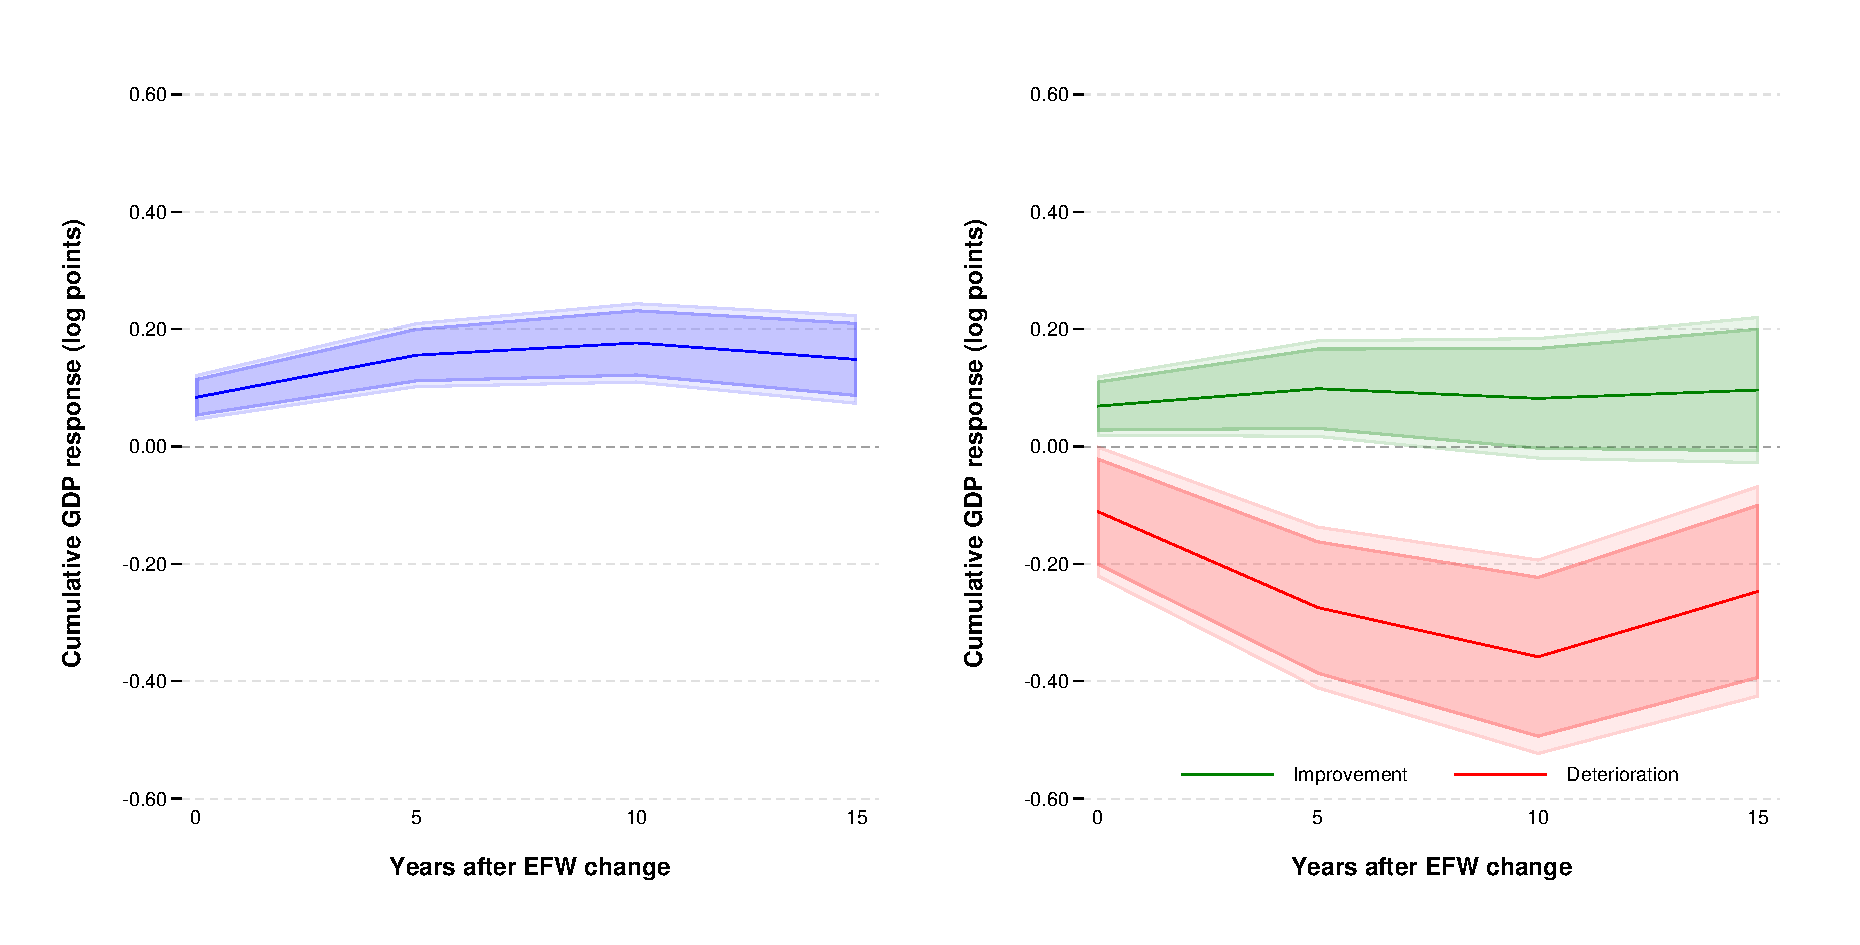
\includegraphics[width=\textwidth,height=7.4cm,keepaspectratio]{../figures/paper_main_figure.pdf}
\end{frame}

% 3 / institutions
\begin{frame}{From economic freedom to \kwTurq{two firm-level channels}}
 \small Economic freedom concerns the ability to use property, make contracts,
 and exchange. The Economic Freedom of the World (EFW) index measures several
 institutional dimensions.\par
 \vspace{2.5mm}
 {\footnotesize\centering
 \renewcommand{\arraystretch}{1.25}
 \begin{tabular}{@{}*{5}{>{\centering\arraybackslash}p{0.174\textwidth}}@{}}
 \toprule
 Area 1 & Area 2 & Area 3 & Area 4 & Area 5\\\midrule
 Size of government & Legal system and property rights & Sound money & Freedom to trade internationally & Regulation\\\bottomrule
 \end{tabular}\par}
 \vspace{3mm}
 \begin{columns}[T,onlytextwidth]
 \begin{column}{0.48\textwidth}
 \labeltext{\kwTurq{$s$: Institutionally usable property}}
 Share of existing property available for productive use under prevailing
 institutional conditions. Title disputes or restrictions on property use
 can make premises unavailable.
 \par\vspace{2mm}\kwOrange{Less usable property: $s\downarrow$}
 \end{column}
 \begin{column}{0.48\textwidth}
 \labeltext{\kwOrange{$c$: Institutional operating overhead}}
 Recurring institutional expenses paid while operating, independently of
 current output: permit renewals and fixed costs of reporting or customs
 administration.
 \par\vspace{2mm}\kwOrange{Higher operating overhead: $c\uparrow$}
 \end{column}
 \end{columns}
 \vspace{3mm}
 {\scriptsize\color{muted}\href{https://efotw.org/economic-freedom/approach}{EFW's five areas: Fraser Institute}}
\end{frame}

% 4 / production
\begin{frame}{From \kwTurq{usable property} to production}
 \begin{columns}[T,onlytextwidth]
 \begin{column}{0.30\textwidth}\panel{pale}{\linewidth}{\centering\labeltext{Fixed property}\[\bar k>0\]\small The firm's existing stock.}\end{column}
 \begin{column}{0.03\textwidth}\vspace{8mm}$\times$\end{column}
 \begin{column}{0.30\textwidth}\panel{pale}{\linewidth}{\centering\labeltext{Usable share}\[s\in(0,1]\]\small Available under institutions.}\end{column}
 \begin{column}{0.03\textwidth}\vspace{8mm}$=$\end{column}
 \begin{column}{0.30\textwidth}\panel{paleteal}{\linewidth}{\centering\labeltext{\kwTurq{Usable property}}\[s\bar k\]\small Available for production.}\end{column}
 \end{columns}
 \vspace{4mm}
 \begin{columns}[T,onlytextwidth]
 \begin{column}{0.48\textwidth}
 \labeltext{1: Combine property with input}
 \small Assume Cobb--Douglas production:
 \[q=A(s\bar k)^{1-\alpha}x^\alpha.\]
 $x\geq0$: variable input.\par
 $A>0$: productivity.\par
 $0<\alpha<1$: output elasticity of $x$.\par
 \vspace{1mm}Output price is one: output equals revenue.
 \end{column}
 \begin{column}{0.48\textwidth}
 \labeltext{2: Choose convenient units}
 \small Measure property in units of the firm's fixed stock: $\bar k=1$.
 \[\boxed{q=As^{1-\alpha}x^\alpha.}\]
 \kwTurq{$s=0.5$:} half the existing stock is available for production.
 \end{column}
 \end{columns}
 \takeaway{An institutional shock changes the usable share $s$. The physical stock $\bar k$ stays fixed.}
\end{frame}

% Baseline and maintained experiment, before the firm problem.
\begin{frame}{One experiment, \kwTurq{one changed assumption}}
 \begin{columns}[T,onlytextwidth]
 \begin{column}{0.48\textwidth}\panel{pale}{\linewidth}{\labeltext{Baseline: free restarting}\[\kappa=0\]}\end{column}
 \begin{column}{0.48\textwidth}\panel{paleteal}{\linewidth}{\labeltext{Extension: costly restarting}\[\kappa>0\]}\end{column}
 \end{columns}
 \vspace{3mm}
 {\centering\small\renewcommand{\arraystretch}{1.3}
 \begin{tabular}{@{}lcc@{}}\toprule
 Institutional path & Shock: $t=0$ & Restored: $t\geq1$\\\midrule
 Deterioration & $s_0-d$ & $s_0$\\
 No change & $s_0$ & $s_0$\\
 Improvement & $s_0+d$ & $s_0$\\\bottomrule
 \end{tabular}\par}
 \vspace{4mm}
 \begin{columns}[T,onlytextwidth]
 \begin{column}{0.48\textwidth}
 \labeltext{Same firm and known restoration}
 \small Initially open; $0<d<s_0$, $s_0+d\leq1$. Restoration is permanent and known at date~0.
 Hold $c=c_0$ and other parameters fixed.
 \end{column}
 \begin{column}{0.48\textwidth}
 \labeltext{What closure means}
 \small Free closure preserves property but dismantles the organization. No organization-preserving suspension;
 financing is available. Discount factor: $0<\beta<1$.
 \end{column}
 \end{columns}
\end{frame}

% 5 / formal-problem
\begin{frame}{The complete \kwTurq{firm problem}}
 \begin{columns}[T,onlytextwidth]
 \begin{column}{0.48\textwidth}
 \labeltext{Activity: $a_t\in\{0,1\}$}
 \small $1$: open. $0$: closed. Initially, $a_{-1}=1$.
 \end{column}
 \begin{column}{0.48\textwidth}
 \labeltext{Variable input: $x_t\geq0$}
 \small Choose input when open; set $x_t=0$ when closed.
 \end{column}
 \end{columns}
 \vspace{3mm}
 \panel{paleteal}{\textwidth}{\labeltext{\kwTurq{Choose activity and input to maximize firm value}}
 \[\max_{\{a_t,x_t\}}\sum_{t=0}^{\infty}\beta^t
 \left[As_t^{1-\alpha}x_t^\alpha-wx_t-(F+c_t)a_t-\kappa a_t(1-a_{t-1})\right].\]}
 \vspace{4mm}
 \begin{columns}[T,onlytextwidth]
 \begin{column}{0.225\textwidth}
 \labeltext{\kwTurq{Revenue}}
 \[As_t^{1-\alpha}x_t^\alpha\]
 \small $A>0$ is productivity. Output price is one.
 \end{column}
 \begin{column}{0.205\textwidth}
 \labeltext{Input bill}
 \[wx_t\]
 \small Input quantity times its fixed unit price $w>0$.
 \end{column}
 \begin{column}{0.25\textwidth}
 \labeltext{Operating overhead}
 \[(F+c_t)a_t\]
 \small $F>0$: ordinary fixed cost.\par
 $c_t\geq0$: institutional overhead. Both paid only when open.
 \end{column}
 \begin{column}{0.255\textwidth}
 \labeltext{\kwOrange{Restart cost}}
 \[\kappa a_t(1-a_{t-1})\]
 \small Pay $\kappa\geq0$ only when closed last period and open now. Otherwise, pay zero.
 \end{column}
 \end{columns}
\end{frame}

% 6 / foc
\begin{frame}{Restart costs leave the \kwTurq{input FOC unchanged}}
 \panel{pale}{\textwidth}{\labeltext{1: Hold the operating decision fixed}
 \small Choose input $x$ to maximize operating profit:
 \[\pi(s,c)=\max_{x\geq0}\{As^{1-\alpha}x^\alpha-wx-F-c\}.\]}
 \vspace{5mm}
 \begin{columns}[T,onlytextwidth]
 \begin{column}{0.47\textwidth}
 \labeltext{2: Differentiate with respect to input}
 \small The slope of operating profit is:
 \[\alpha As^{1-\alpha}x^{\alpha-1}-w.\]
 One extra unit adds revenue and costs $w$.
 \end{column}
 \begin{column}{0.49\textwidth}
 \labeltext{\kwTurq{3: Set the slope equal to zero}}
 \small The first-order condition is:
 \[\boxed{\alpha As^{1-\alpha}x^{\alpha-1}=w.}\]
 Marginal revenue product = input price.
 \end{column}
 \end{columns}
 \vspace{3mm}
 \takeaway{Diminishing returns give a unique optimum. The FOC is unchanged: rebuilding costs do not depend on $x$. The changed result concerns closure and recovery.}
\end{frame}

% 7 / solution
\begin{frame}{From \kwTurq{optimal input} to output and profit}
 \begin{columns}[c,onlytextwidth]
 \begin{column}{0.38\textwidth}
 \labeltext{1: Choose input}
 \small Rearrange the FOC, then raise both sides to $1/(1-\alpha)$.
 \end{column}
 \begin{column}{0.59\textwidth}
 \[\begin{aligned}x^{1-\alpha}&=\frac{\alpha As^{1-\alpha}}{w},\\
 x^*(s)&=s\left(\frac{\alpha A}{w}\right)^{1/(1-\alpha)}.\end{aligned}\]
 \end{column}
 \end{columns}
 \vspace{1mm}{\color{line}\hrule}\vspace{2mm}
 \begin{columns}[c,onlytextwidth]
 \begin{column}{0.38\textwidth}
 \labeltext{2: Compute output}
 \small Substitute optimal input into production.
 \end{column}
 \begin{column}{0.59\textwidth}
 \[q(s)=sA\left(\frac{\alpha A}{w}\right)^{\alpha/(1-\alpha)}.\]
 \end{column}
 \end{columns}
 \vspace{2mm}{\color{line}\hrule}\vspace{2mm}
 \begin{columns}[c,onlytextwidth]
 \begin{column}{0.38\textwidth}
 \labeltext{\kwTurq{3: Compute operating profit}}
 \small Multiply the FOC by $x^*$:\par input spending is $wx^*=\alpha q$.
 \end{column}
 \begin{column}{0.59\textwidth}
 \[\begin{aligned}\pi(s,c)&=q(s)-wx^*(s)-F-c\\&=(1-\alpha)q(s)-F-c.\end{aligned}\]
 \end{column}
 \end{columns}
 \takeaway{$q(s_t)$ is output if operating. Actual output is $y_t=a_tq(s_t)$: $a_t=1$ if open and $0$ if closed.}
\end{frame}

% 8 / channels: static comparison of the interactive presets.
\begin{frame}{Two channels, \kwTurq{different effects}}
 \centering
 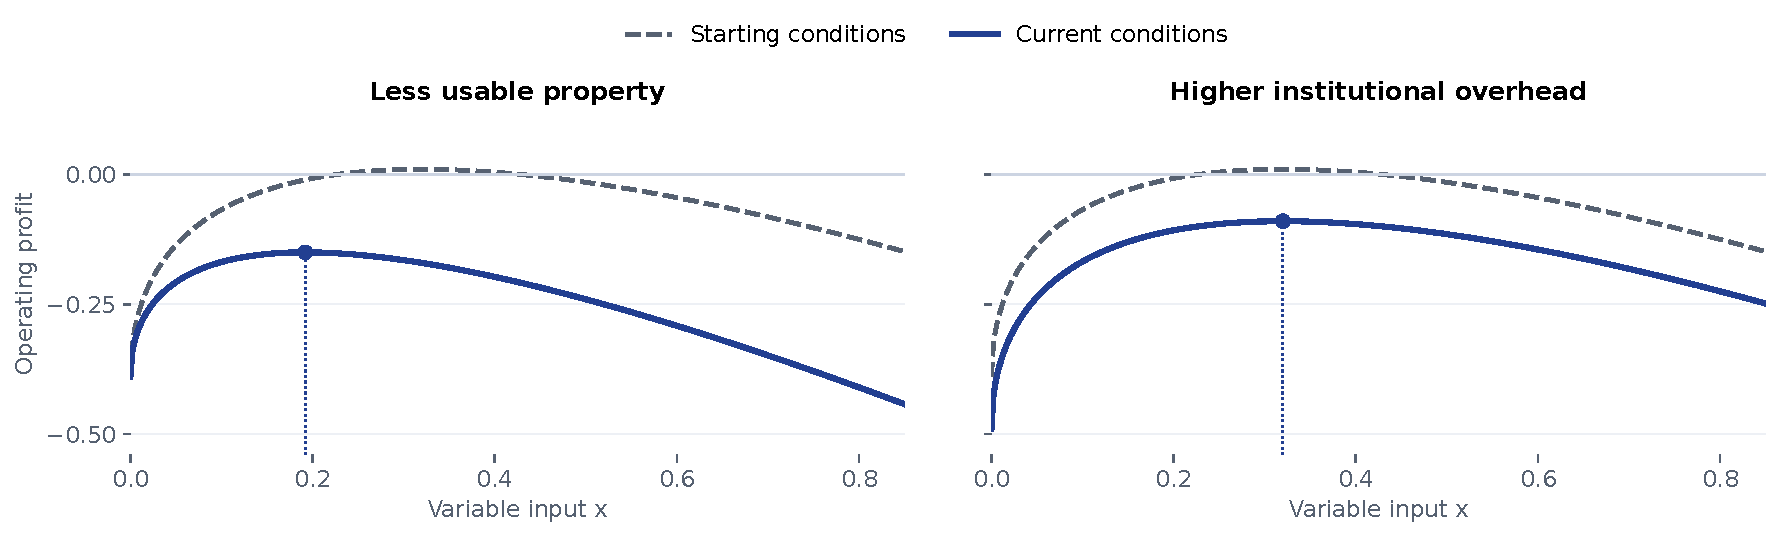
\includegraphics[width=\textwidth,height=4.2cm,keepaspectratio]{figures/channel_profit.pdf}\par
 \vspace{1mm}
 {\small\renewcommand{\arraystretch}{1.18}
 \begin{tabular}{@{}lrrr@{}}
 \toprule
 Conditional on operating & Starting & Lower $s$ & Higher $c$\\\midrule
 Chosen input $x^*$ & 0.320 & 0.192 & 0.320\\
 Output $q$ & 0.80 & 0.48 & 0.80\\
 Operating profit $\pi$ & 0.01 & $-0.15$ & $-0.09$\\\bottomrule
 \end{tabular}\par}
 \takeaway{Less usable property changes optimal input and output. Higher overhead shifts profit vertically without changing either operating choice.}
 {\scriptsize\color{muted}Illustrative values: $s:0.50\to0.30$ or $c:0.09\to0.19$, one change at a time.}
\end{frame}

% 9 / closure
\begin{frame}{\kwOrange{Closure today} and \kwTurq{restarting later}}
 \begin{columns}[T,onlytextwidth]
 \begin{column}{0.30\textwidth}\panel{pale}{\linewidth}{\labeltext{Normal operating profit}\[\pi_0=\pi(s_0,c_0)>0\]}\end{column}
 \begin{column}{0.32\textwidth}\panel{pale}{\linewidth}{\labeltext{\kwOrange{Deterioration profit}}\[\pi_-=\pi(s_0-d,c_0)\]}\end{column}
 \begin{column}{0.34\textwidth}\panel{paleteal}{\linewidth}{\labeltext{\kwTurq{Normal business value}}\[V=\frac{\pi_0}{1-\beta},\quad 0<\beta<1\]}\end{column}
 \end{columns}
 \vspace{4mm}
 \begin{columns}[T,onlytextwidth]
 \begin{column}{0.48\textwidth}
 \labeltext{\kwTurq{Keep operating}}
 \[\pi_-+\beta V\]
 \small Current profit plus discounted future earnings.
 \end{column}
 \begin{column}{0.48\textwidth}
 \labeltext{\kwOrange{Close now}}
 \[\beta\max\{V-\kappa,0\}\]
 \small Closure is free; restarting remains an option.
 \end{column}
 \end{columns}
 \vspace{4mm}{\color{line}\hrule}\vspace{3mm}
 \begin{columns}[T,onlytextwidth]
 \begin{column}{0.48\textwidth}
 \labeltext{After institutions are restored}
 \small Closure preserves property but dismantles the organization.
 Rebuilding the workforce and commercial relationships costs $\kappa$.
 \end{column}
 \begin{column}{0.48\textwidth}
 \labeltext{Net value of restarting: $V-\kappa$}
 \panel{paleteal}{0.47\linewidth}{\centering\kwTurq{$V>\kappa$}\par\small Restart}
 \hfill\panel{paleorange}{0.49\linewidth}{\centering\kwOrange{$V<\kappa$}\par\small Remain closed}
 \end{column}
 \end{columns}
\end{frame}

% 10 / conjecture
\begin{frame}{Conjecture: a temporary setback, a \kwOrange{lasting loss}}
 \small Maintain the experiment and assumptions above.\par\vspace{1mm}
 \labeltext{1: Conditions \hfill\normalfont\small Improvement profit: $\pi_+=\pi(s_0+d,c_0)$}
 \begin{columns}[T,onlytextwidth]
 \begin{column}{0.31\textwidth}
 \panel{pale}{\linewidth}{\small\textbf{Normal operation pays}\[\pi_0>0\]\small Positive operating profit under normal conditions.}
 \end{column}
 \begin{column}{0.31\textwidth}
 \panel{pale}{\linewidth}{\small\textbf{Continuation loses value}\[\pi_-+\beta V<0\]\small Future earnings cannot offset the current loss.}
 \end{column}
 \begin{column}{0.34\textwidth}
 \panel{pale}{\linewidth}{\small\textbf{Rebuilding is too costly}\[\kappa>\pi_++\beta V\]\small An identical inactive owner would not enter even during improvement.}
 \end{column}
 \end{columns}
 \vspace{4mm}
 \begin{columns}[T,onlytextwidth]
 \begin{column}{0.42\textwidth}
 \labeltext{2: Decisions}
 \small\kwOrange{Deterioration}\par Close and never restart.\par\vspace{3mm}
 \kwTurq{Improvement or no change}\par Remain open.
 \end{column}
 \begin{column}{0.55\textwidth}
 \labeltext{3: Output comparison}
 \small Normal output: $q_0=q(s_0)$.\par Loss and gain are relative to no change.
 \vspace{1mm}
 \renewcommand{\arraystretch}{1.3}
 \begin{tabular}{@{}lcc@{}}\toprule
 When? & \kwOrange{Loss} & \kwTurq{Gain}\\\midrule
 During the shock & $q_0$ & $(d/s_0)q_0$\\
 After restoration & $q_0$ & $0$\\\bottomrule
 \end{tabular}
 \end{column}
 \end{columns}
 \takeaway{Because $d<s_0$, the initial loss exceeds the gain. After restoration, the loss persists while the gain disappears.}
\end{frame}

% 11 / experiment: all three interactive cases on one static chart.
\begin{frame}{\kwTurq{Institutions recover}. Does production recover too?}
 \centering
 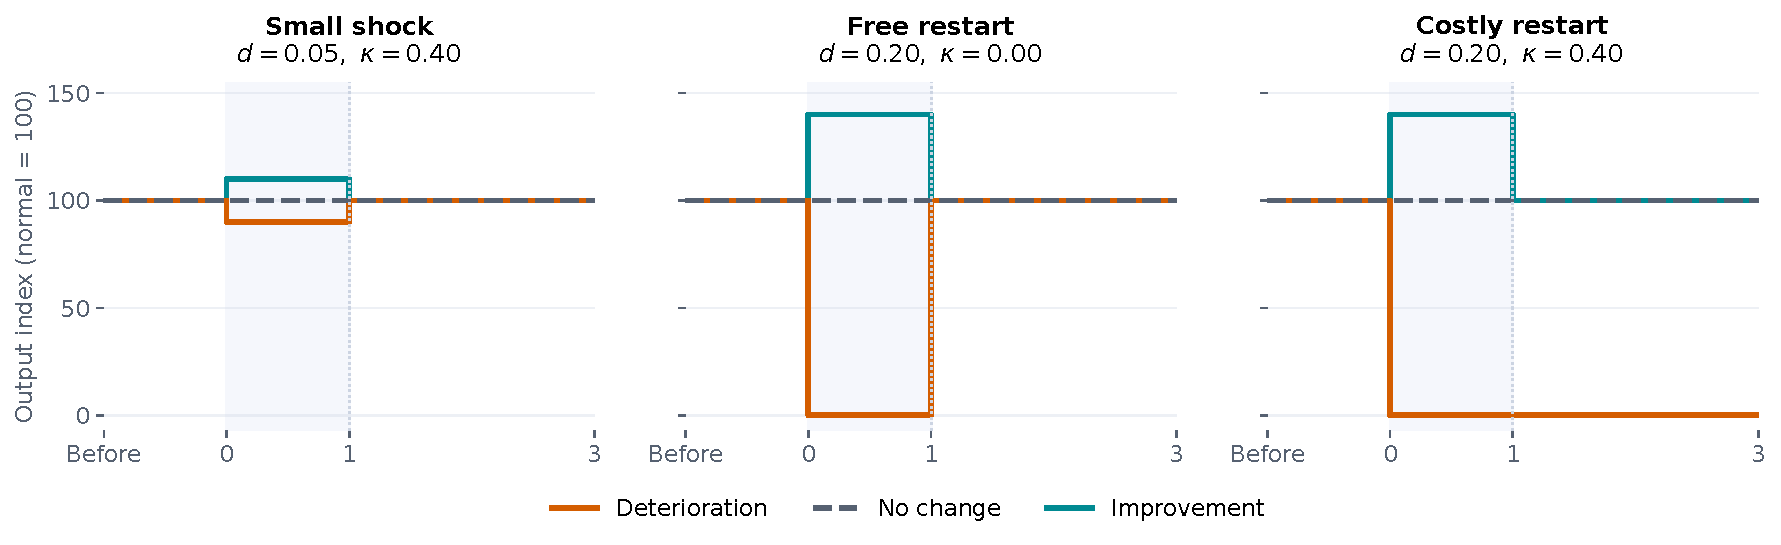
\includegraphics[width=\textwidth,height=4.8cm,keepaspectratio]{figures/output_cases.pdf}\par
 {\small Before the shock\quad$\longrightarrow$\quad Temporary shock: $t=0$\quad$\longrightarrow$\quad Restored: $t\geq1$}\par
 \vspace{3mm}
 \begin{columns}[T,onlytextwidth]
 \begin{column}{0.31\textwidth}\panel{pale}{\linewidth}{\labeltext{Small shock}\small Open $\to$ open $\to$ open.}
 \end{column}
 \begin{column}{0.31\textwidth}\panel{paleteal}{\linewidth}{\labeltext{\kwTurq{Free restart}}\small Open $\to$ close $\to$ reopen.}
 \end{column}
 \begin{column}{0.34\textwidth}\panel{paleorange}{\linewidth}{\labeltext{\kwOrange{Costly restart}}\small Open $\to$ close $\to$ stay closed.}
 \end{column}
 \end{columns}
 \takeaway{The last two cases use the same shock. Only the restart cost changes.}
\end{frame}

\begin{frame}{Prior work and \kwTurq{my proposed contribution}}
 \begin{columns}[T,onlytextwidth]
 \begin{column}{0.48\textwidth}
 \labeltext{Established mechanism}
 \small \href{https://doi.org/10.1086/261619}{Dixit (1989), pp.~621, 623, 629}: organizational decay,
 temporary reversals, and tolerating losses to avoid rebuilding.\par\vspace{3mm}
 \href{https://doi.org/10.1257/jep.6.1.107}{Dixit (1992), pp.~119--120}: suspension differs from abandonment.
 Its appendix (pp.~129--131) sets out the stochastic switching equations.\par\vspace{3mm}
 \href{https://pure.psu.edu/en/publications/the-decision-to-export-in-colombia-an-empirical-model-of-entry-wi/}{Roberts and Tybout (1997)}: evidence of sunk entry costs in exporting;
 not a test of EFW shocks. Review limited to the author-institution abstract.
 \end{column}
 \begin{column}{0.48\textwidth}
 \labeltext{Scope of the literature review}
 \small Dixit's pp.~625 and 630 refer to appendices A/B available from the author;
 the published article does not include them.\par\vspace{4mm}
 \href{https://econpapers.repec.org/RePEc:fth:prinec:91}{Princeton paper~91 (1988)} is catalogued,
 with no downloadable text there. Their contents remain outside this review.
 \end{column}
 \end{columns}
 \vspace{4mm}
 \takeaway{I retain costly rebuilding and use known institutional paths to derive the conditional loss--gain comparison.
 I will then test suspension and entry. This bounded review does not establish originality.}
\end{frame}

% 12 / research
\begin{frame}{The mechanism and \kwTurq{next steps}}
 \begin{columns}[T,onlytextwidth]
 \begin{column}{0.31\textwidth}\panel{pale}{\linewidth}{\labeltext{Institutions}\small Usable property and overhead change profitability.}\end{column}
 \begin{column}{0.31\textwidth}\panel{pale}{\linewidth}{\labeltext{\kwOrange{Activity}}\small Equal shocks can produce different closure decisions.}\end{column}
 \begin{column}{0.34\textwidth}\panel{pale}{\linewidth}{\labeltext{\kwTurq{Persistence}}\small Costly restarting can prevent output recovery.}\end{column}
 \end{columns}
 \vspace{4mm}
 \begin{columns}[T,onlytextwidth]
 \begin{column}{0.31\textwidth}
 \labeltext{Prove by hand}
 \small Input optimum; value comparisons for operating, closing, and restarting;
 conditional output inequalities.
 \end{column}
 \begin{column}{0.31\textwidth}
 \labeltext{\kwOrange{Simulate}}
 \small Vary margins, shock size and duration, and restart costs. Allow suspension,
 entry, and heterogeneous firms.
 \end{column}
 \begin{column}{0.34\textwidth}
 \labeltext{Formalize in Lean}
 \small Optimizer and value identities; switching rules and no delayed reentry;
 conditional inequalities, with logs only for positive output.
 \end{column}
 \end{columns}
 \vspace{4mm}
 \panel{paleorange}{\textwidth}{\labeltext{\kwOrange{The step most likely to fail}}
 \small A temporary shock may induce \textbf{cheap suspension}, without dismantling
 the organization and requiring costly rebuilding.}\par
 \vspace{3mm}
\end{frame}
\end{document}
